\chapter{创新性与应用前景}

本作品围绕格IB-ME完整运行中的三个主要问题开展优化：大规模相关采样需要大量内存，密钥和
签名的文本表示占用较多空间，固定身份通信重复执行委派。结构化环采样、范围感知编码和接收
会话复用分别从计算结构、数据表示和处理时机入手，使不同格原语能够共同支持消息收发。

\section{结构化环采样的内存优化}

Sageloli身份签名需要由大规模陷门生成相关扰动。若将环多项式展开为系数空间中的稠密矩阵，
PARAM-I的单个双精度矩阵就需要约1.18~TiB，相关矩阵的分解和乘法还要处理数量庞大的元素。
这一开销直接影响目标规模下的发钥和签名。

本作品保留陷门的多项式表示，利用负循环Fourier变换将环运算分解到各频率，再利用协方差修正项的
低秩性质计算平方根作用。PARAM-I在每个频率上分解$65\times65$的Gram矩阵；陷门系数、频域
表示和小矩阵分解结果共同构成采样所需的数据。计算时通过小矩阵与向量乘法生成相关扰动，随后
完成系数域中的离散采样。

这项优化将存储规模组织为$O(d\ell k+dk^2)$，使环结构贯穿发钥和签名过程。
PARAM-I与PARAM-II均完成发钥、签名和公开验证，实测峰值RSS分别约为1.36与6.19~GiB。
由此，大参数环格身份签名可以在数GiB内存中执行，并进一步用于完整IB-ME消息认证。

\section{按取值范围压缩密钥与签名}

SRGG公钥、机构状态、用户密钥和签名包含不同范围的整数。使用JSON时，整数的十进制字符、
负号及分隔符共同增加文件长度，机构向多个用户分发密钥、系统保存主陷门及传输签名时都会承担
这些开销。

本作品按字段的数学取值范围选择位数，并为各类对象规定统一编码。例如，三值陷门系数用2~bit
表示，二元挑战用1~bit表示，模$Q$公开系数用24~bit表示；短密钥和响应先处理符号，再按所需位数
写入。对象头部记录类型、参数和身份信息，接收端据此恢复系数数组与数学对象。

三组SRGG参数的机构状态压缩到原JSON长度的18.3\%至19.8\%，签名压缩到37.7\%至39.1\%。
在LATTE＋SRGG PARAM-I的10字节消息运行中，签名长度减少约62.0\%，完整密文长度减少约12.8\%。
这项优化同时作用于长期密钥保存和逐消息传输：前者降低机构与用户的存储需求，后者直接缩短
对称加密内容。统一编码还使密钥文件与传输对象共享同一套加载过程。

\section{固定身份通信的接收会话复用}

两层HIBE接收端先根据接收身份和认可发送身份生成叶密钥，再恢复消息。连续通信中，双方身份
和系统公钥通常在一段时间内保持固定，叶密钥适用于这一身份路径。Lai完整解密的阶段分解显示，
二级委派约占92.5\%，反复执行委派成为连续接收时的主要成本。

本作品将叶密钥生成安排在会话准备阶段，并把叶密钥与系统公钥、双方身份及组合配置一起保存于
会话对象。后续密文进入同一会话后，使用已准备的叶密钥完成解密和发送身份认证。机构可以在
通信开始前准备会话，在多个接收任务之间复用相应的身份路径。

会话实验中，单条原路径解密约526秒；准备约510秒后，会话内解密中位数约28.6秒，提速约
18.4倍，耗时减少约94.6\%。叶密钥编码长度约34.7~MiB。这一安排把较集中的计算放到服务
启动或通信建立阶段，降低后续每条消息的等待时间，适合固定机构间的持续数据交换。

\section{多算法组合与业务集成}

三项优化通过同一套协议服务于完整消息收发。系统将HIBE与IBS分别接入，组合配置记录各自的
参数、身份长度、消息容量和对象格式。两种HIBE与五种常规IBS形成十种组合，应用通过相同的
密钥生成、消息加密和匹配解密操作选择不同算法。

这一组织方式使新增原语能够沿用已有应用流程。HIBE明文容量较小时，短种子封装把其加密输入
固定为32字节；IBS签名较大时，消息容量按签名长度与加密内容上限计算。原语之间的参数与
对象差异由组合配置描述，命令行、浏览器和状态恢复继续使用公共协议。

Wang--PW接入进一步扩展了系统可处理的对象规模。其公钥约64.0~MiB，用户签名密钥约2.06~GiB，
签名约384~KiB；后端通过密钥文件的保存与加载接入LATTE，完成独立签验及完整消息收发。
机构可将Wang--PW的发钥与签名安排在服务器上，消息收发继续使用现有应用入口。



算法迁移可按业务逐步开展。组合配置明确算法名称、参数和对象版本，业务服务可先建立新组合
的系统公钥与角色密钥，再将新消息切换到相应组合；已经保存的密文按其组合标识使用对应配置
和密钥。应用通过统一的发送与接收操作衔接不同组合，逐步调整机构和用户的运行环境。

在现有业务系统中，发钥服务可对接组织目录或设备台账，消息服务负责传递规范密文字节，
文件服务保存角色密钥与加密文件。交互式应用采用响应较快的组合，后台任务按计划完成签名，
固定机构间通信复用接收会话。算法选择因而可以与实际的消息时效、发送频率和服务器资源相配合。

\section{应用前景}

IB-ME将接收身份和认可的发送身份共同用于消息恢复，适合通信角色明确、由机构统一管理身份
密钥的业务。以下结合消息时效、发送端计算与通信频率，说明三类应用方式。

\subsection{机构定向消息与跨部门协作}

单位内部的通知、审批反馈、值班指令和受控资料具有明确的发送部门与接收岗位。以安全管理部门
向区域值班负责人发送处置指令为例，机构为部门签发发送方密钥，为岗位签发接收方密钥。部门
加密时指定岗位身份，负责人接收时指定认可的部门身份，两项匹配后恢复指令。

机构按组织目录核验领钥者，将部门、岗位和有效期编入身份字符串。密文由内部文件服务或
消息队列传递；A组用于交互式工作台，B组由发送队列完成批量通知、审批结果和访问凭据投递。

\begin{figure}[!htbp]
\centering
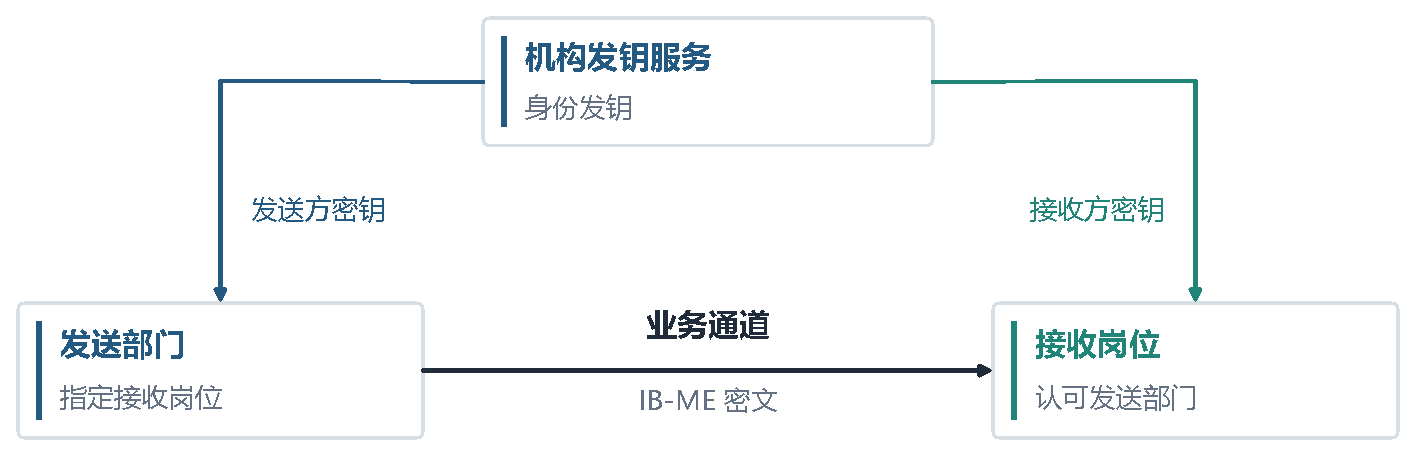
\includegraphics[width=\linewidth,height=.62\textheight,keepaspectratio]{figures/fig-08-01-application.pdf}
\caption{机构定向消息中的身份签发与密文流转}
\label{fig:institutional-message}
\end{figure}

\subsection{受控终端与设备指令分发}

管理平台向终端发送配置、更新通知或操作指令时，既要指定接收设备，也要让设备识别认可的
管理身份。可将设备编号、区域和用途组成接收身份，将控制服务或管理部门名称组成发送身份。
设备网关根据自身接收方密钥和预设的管理身份恢复指令，再交由业务程序处理。

A组适合需要及时返回处理结果的操作，B组适合由管理平台提前生成的批量配置和定向凭据。
密码处理可部署在具备相应内存的设备网关，终端通过既有管理通道取得处理后的业务命令。


\subsection{固定机构间周期报送}

分支机构向管理中心按小时或按日报送设备摘要、巡检结果和业务核对信息时，双方身份长期固定，
报送时机也相对明确。C组可在接收服务启动时为各报送方准备会话，将委派计算安排在报送窗口
之前；收到消息后，管理中心使用对应的叶密钥解密，并核对发送机构身份。

单条3,924字节的应用容量可承载结构化状态、统计摘要和校验结果，约4.34~MiB的完整密文通过
机构网络传输。接收中心保存每个固定对端的会话状态，按计划处理连续消息；双方身份或系统
公钥更新时，建立相应的新会话。这种处理方式适用于具有稳定网络和服务器资源的机构间交换。
